\documentclass[12pt]{article}
\usepackage[utf8]{inputenc}
\usepackage[T1]{fontenc}
\usepackage[polish]{babel}
\usepackage{polski}
\usepackage{indentfirst}
\usepackage{hyperref}
\usepackage{graphicx}
\usepackage{float}
\usepackage{amsmath}
\usepackage{xurl}
\usepackage{tabularx}
\usepackage{minted}
\usepackage{subfigure}
\usepackage[section]{placeins}
\usepackage{subfiles}


\usepackage{pifont}
\newcommand{\cmark}{\ding{52}}%
\newcommand{\xmark}{\ding{53}}%


\textheight 23.2 cm

\textwidth 6.0 in

\hoffset = -0.5 in

\voffset = -2.4 cm
\title{Dokumentacja końcowa projektu \\
\large{Programowanie aplikacji mobilnych w technologii Flutter}}

\author{Michał Szeląg}
\date{Kwiecień 2023}

\begin{document}

\maketitle

\section{Opis Projektu}
% QR na dołączenie do pokoju
Projekt ma symulować rozgrywkę dla wielu graczy (od 5 do 10) w stylu gry planszowej "The Resistance: Avalon". Celem aplikacji jest ułatwienie przeprowadzenia sesji gry w przypadku braku lub niepełnej kopii fizycznej gry jako rozgrywkę w stylu local-multiplayer. 

Gracze są losowo dzieleni na dobrych i złych - źli powinni na początku rozgrywki poznać innych złych, dobrzy nie wiedzą nic na pewno aż do końca gry.
Rozgrywka polega na wyborze drużyn, które wysłane zostaną na misje. Drużyny wybierają wszyscy gracze (tj. jeden wybiera, pozostali głosują - wystarczy zwykła większość). Na każdą z pięciu misji trzeba wybrać inna ilość osób do drużyny. Gracz wybrany do drużyny w sposób tajny głosuje za powodzeniem misji: dobry musi wybrać sukces, a zły ma do wyboru sukces lub porażkę. Wystarczy jeden głos za porażką aby misja się nie powiodła. 

Dobrzy wygrywają jeśli 3 z 5-ciu misji się powiodły, a Źli jeśli 3 z 5-ciu misji się nie powiodły.
\\\\
Jedna sesja gry przebiega następująco:
\begin{itemize}
    \item Założenie pokoju przez jednego z graczy(hosta).
    \item Dołączanie graczy do pokoju - gracze mogą dołączać do pokoju poprzez podanie kodu sesji. Host widzi listę graczy znajdujących się w pokoju i może ją modyfikować - wyrzucać graczy z pokoju.
    \item Wybór postaci w grze - host wybiera wersję rozgrywki, tj. postaci, które mogą zostać przydzielone graczom. Możliwa jest gra bez postaci.
    \item Losowanie ról - każdy z graczy w tajny sposób dowiaduje się czy w tej rozgrywce będzie wcielać się w złego czy dobrego. Dodatkowa informacja dla złych, o tym kim są pozostali źli, wyświetlana jest teraz. Losowany jest także gracz rozpoczynający rozgrywkę - Przywódca.
    \item Start gry: \begin{enumerate}
        \item Przywódca wybiera z listy graczy, tych którzy wybiorą się na misję - inni gracze mogą zobaczyć na swoim ekranie, kogo wybrał Przywódca.
        \item Głosowanie na drużynę (jawne) - wszyscy gracze głosują czy zgadzają się, aby ta drużyna poszła na misję. Jeśli drużyna nie zostanie wybrana następuje zmiana przywódcy na kolejnego z listy. Piąta z kolei niewybrana drużyna oznacza wygraną złych.
        \item Głosowanie na misji (tajne) - gracze wybrani do drużyny głosują za powodzeniem bądź porażką misji. Aby inni nie mogli się domyśleć na co zagłosowali opcje 'sukces' i 'porażka' będą w losowy sposób umiejscowione na ekranie głosowania.
        \item Wynik misji - Gracze dowiadują się jaki jest wynik misji. Potem następuje zmiana Przywódcy na kolejną osobę z listy.
    \end{enumerate}
    \item Koniec gry - po trzech misjach udanych lub trzech udanych następuje rozstrzygnięcie wyniku gry. W tym momencie dostępna powinna być akcja związana z dodatkowymi postaciami, mogąca zmienić wynik gry.
\end{itemize}


\section{Integracje}
Projekt nie jest zintegrowany z żadną zewnętrzną aplikacją. Korzysta z Firebase Authentication i Firebase Firestore Database.

\section{Lista wymagań opcjonalnych}

\begin{table}[H]
\centering
\begin{tabular}{|l|c|c|}
    \hline 
    Support for Android & 5pt
    & \cmark
    \\\hline
    Support for iOS & 5pt
    & \xmark(?)
    \\\hline
    Support for Web & 5pt
    & \cmark
    \\\hline
    Support for Desktop & 5pt
    & \xmark
    \\\hline
    Implementing BLoC pattern & 10pt
    & \cmark
    \\\hline
    Animations & 10pt
    & \xmark
    \\\hline
    Tests & 10pt
    & \xmark
    \\\hline
    Signing in process & 10pt
    & \cmark
    \\\hline
    Complex form with validation & 10pt
    & \cmark
    \\\hline
    CI/CD & 5pt
    & \cmark
    \\\hline
    Platform Channels & 10pt
    & \xmark
    \\\hline
    Accessibility & 5pt
    & \xmark
    \\\hline
    Internationalization & 5pt
    & \cmark
    \\\hline
    Offline support & 20pt
    & \xmark
    \\\hline
    Custom painting & 10pt
    & \xmark
    \\\hline
    Deep links & 10pt
    & \xmark
    \\\hline
    Other platform features & 10pt
    & \xmark
    \\\hline
\end{tabular}
\end{table}














\newpage
\section{Instrukcja}
Na większości urządzeń aplikacja nie zajmuje całego ekranu - należy przejść do ustawień urządzenia i dodać aplikacji zezwolenie na tryb pełnoekranowy, jednak nie wpływa to na jej działanie.
\subsection{Logowanie}
Po zainstalowaniu i uruchomieniu aplikacji użytkownik witany jest poniżym ekranem:
\begin{figure}[!htb]
    \centering
    \subfigure{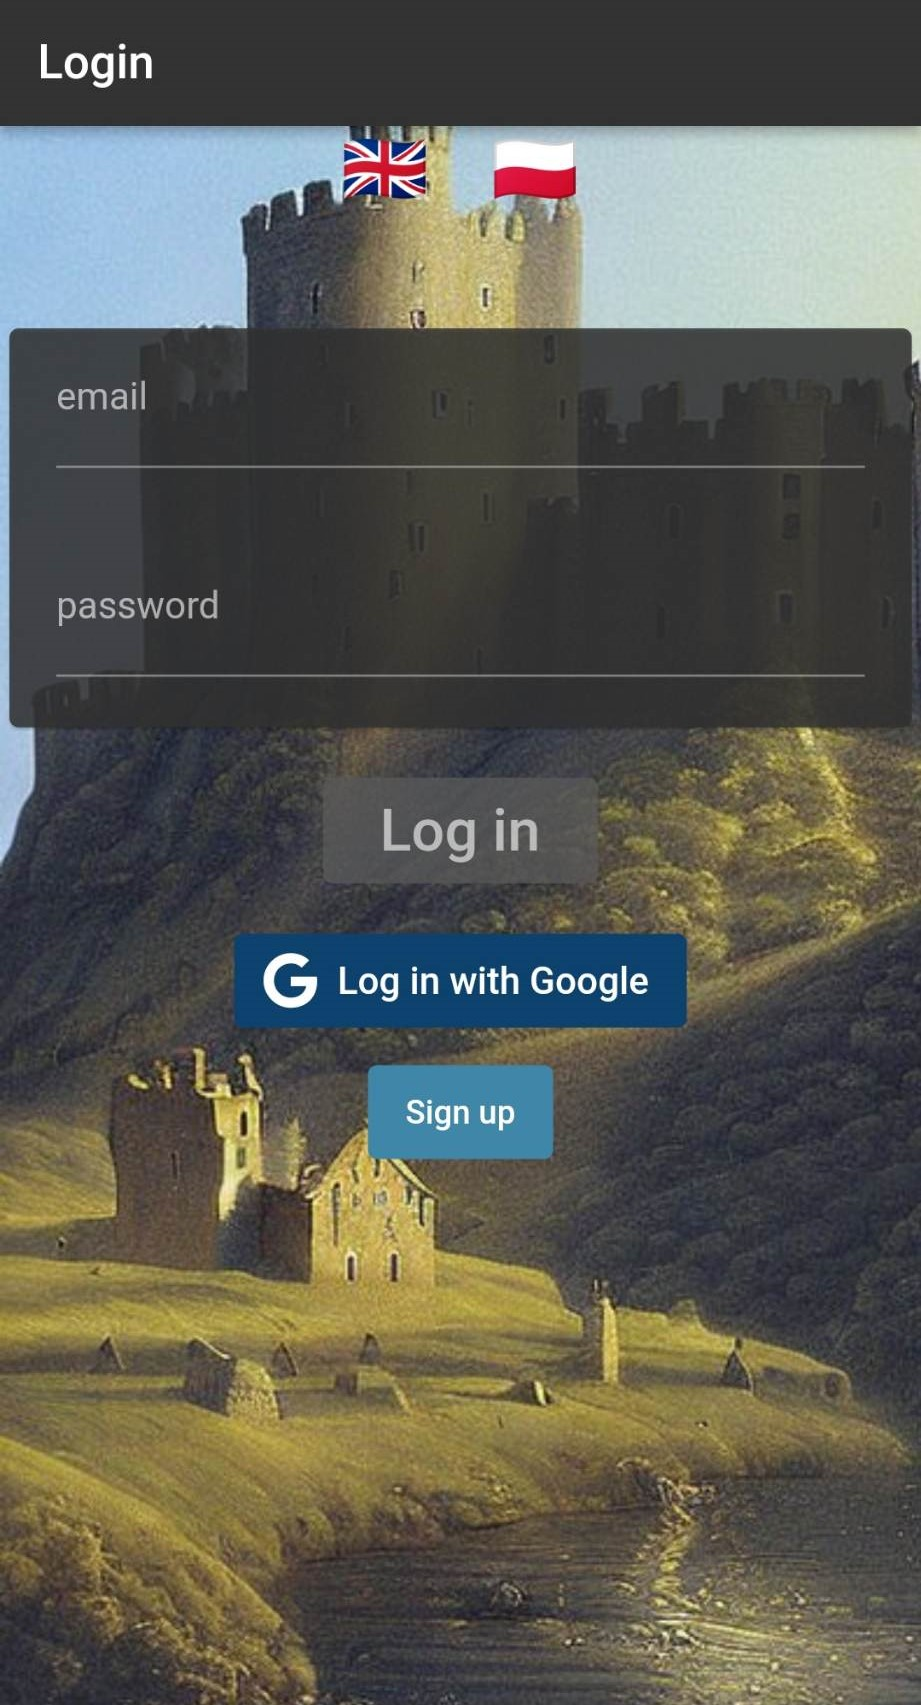
\includegraphics[width=0.4\textwidth]{./img/login.jpg}} 
    \subfigure{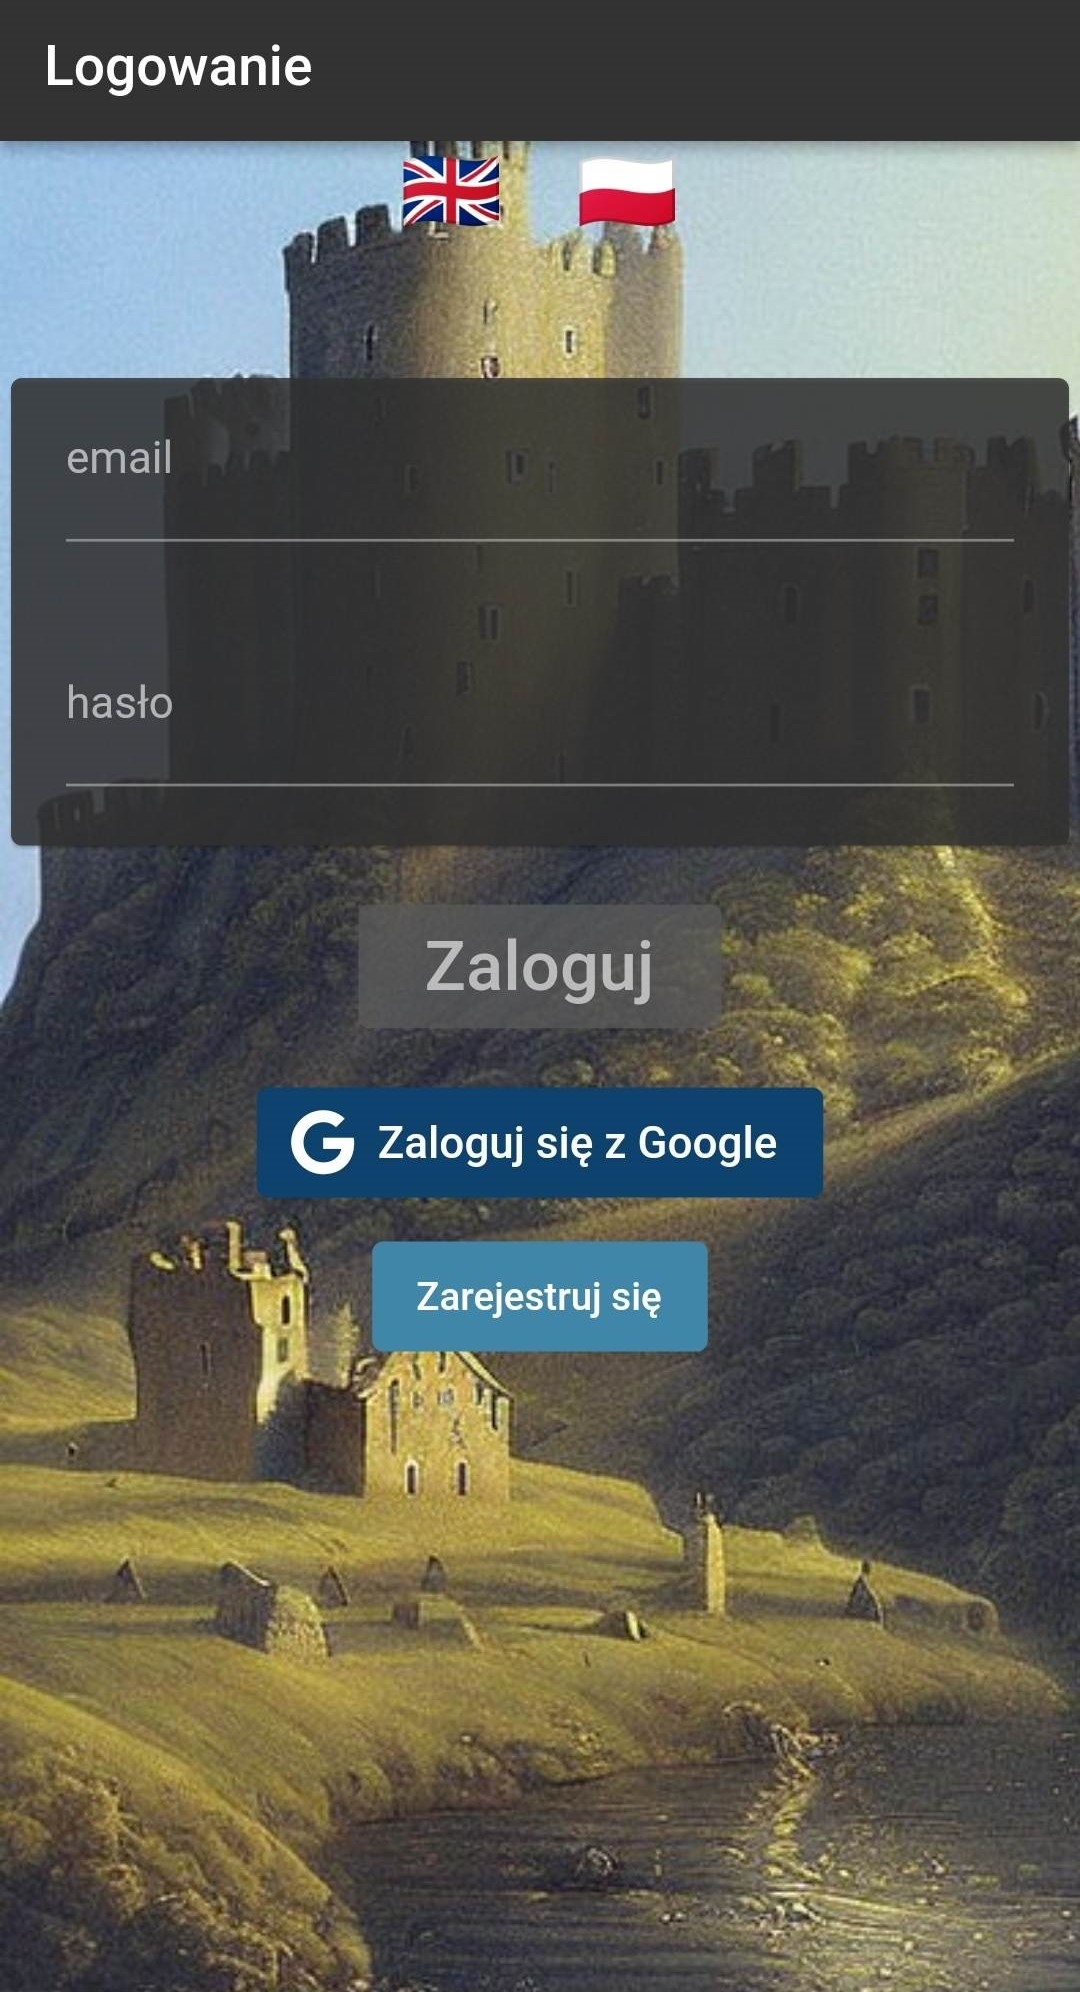
\includegraphics[width=0.4\textwidth]{./img/loginpl.jpg}} 
    \centering
\end{figure}
Użytkownik może:
\begin{itemize}
    \item zmieniać język aplikacji między polskim i angielskim za pomocą przycisków na górze ekranu z flagami. 
    \item zalogować się używając wcześniej zarejestrowanego email'a i hasła
    \item zalogować się z kontem Google
    \item przejść do ekranu rejestracji
\end{itemize}
Pola tekstowe email i hasło podlegają walidacji.

\newpage
\subsection{Rejestracja}
Jeśli użytkownik chce utworzyć nowe konto przechodzi do ekranu rejestracji:
\begin{figure}[!htb]
    \centering
    \subfigure{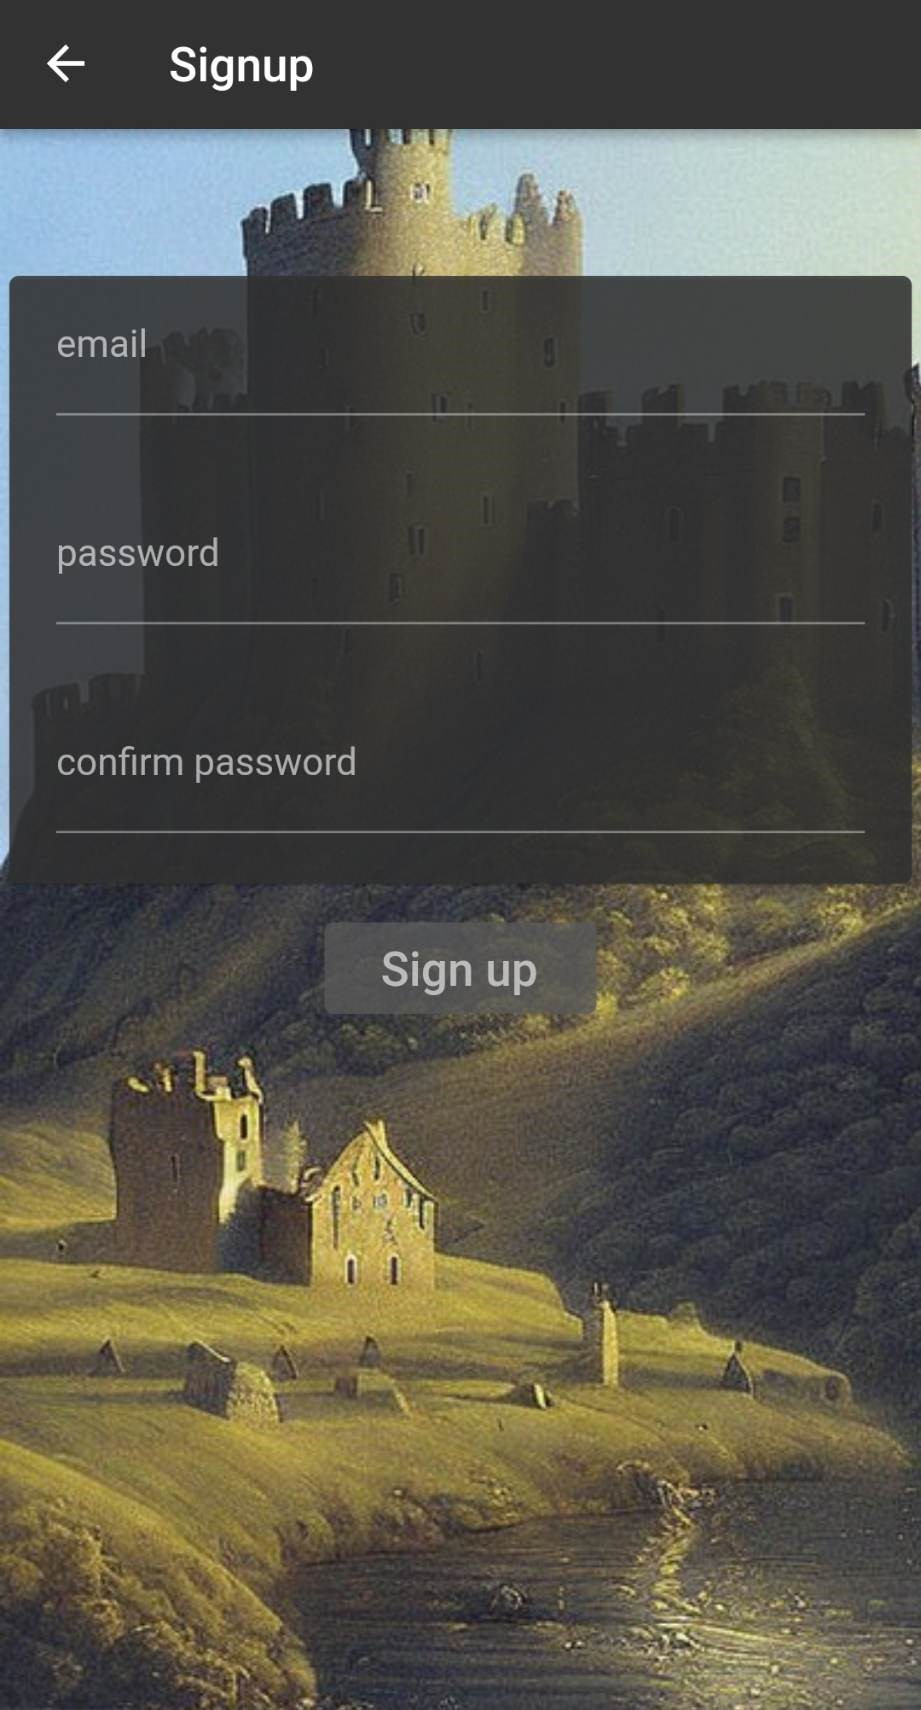
\includegraphics[width=0.4\textwidth]{./img/signup1.jpg}} 
    \subfigure{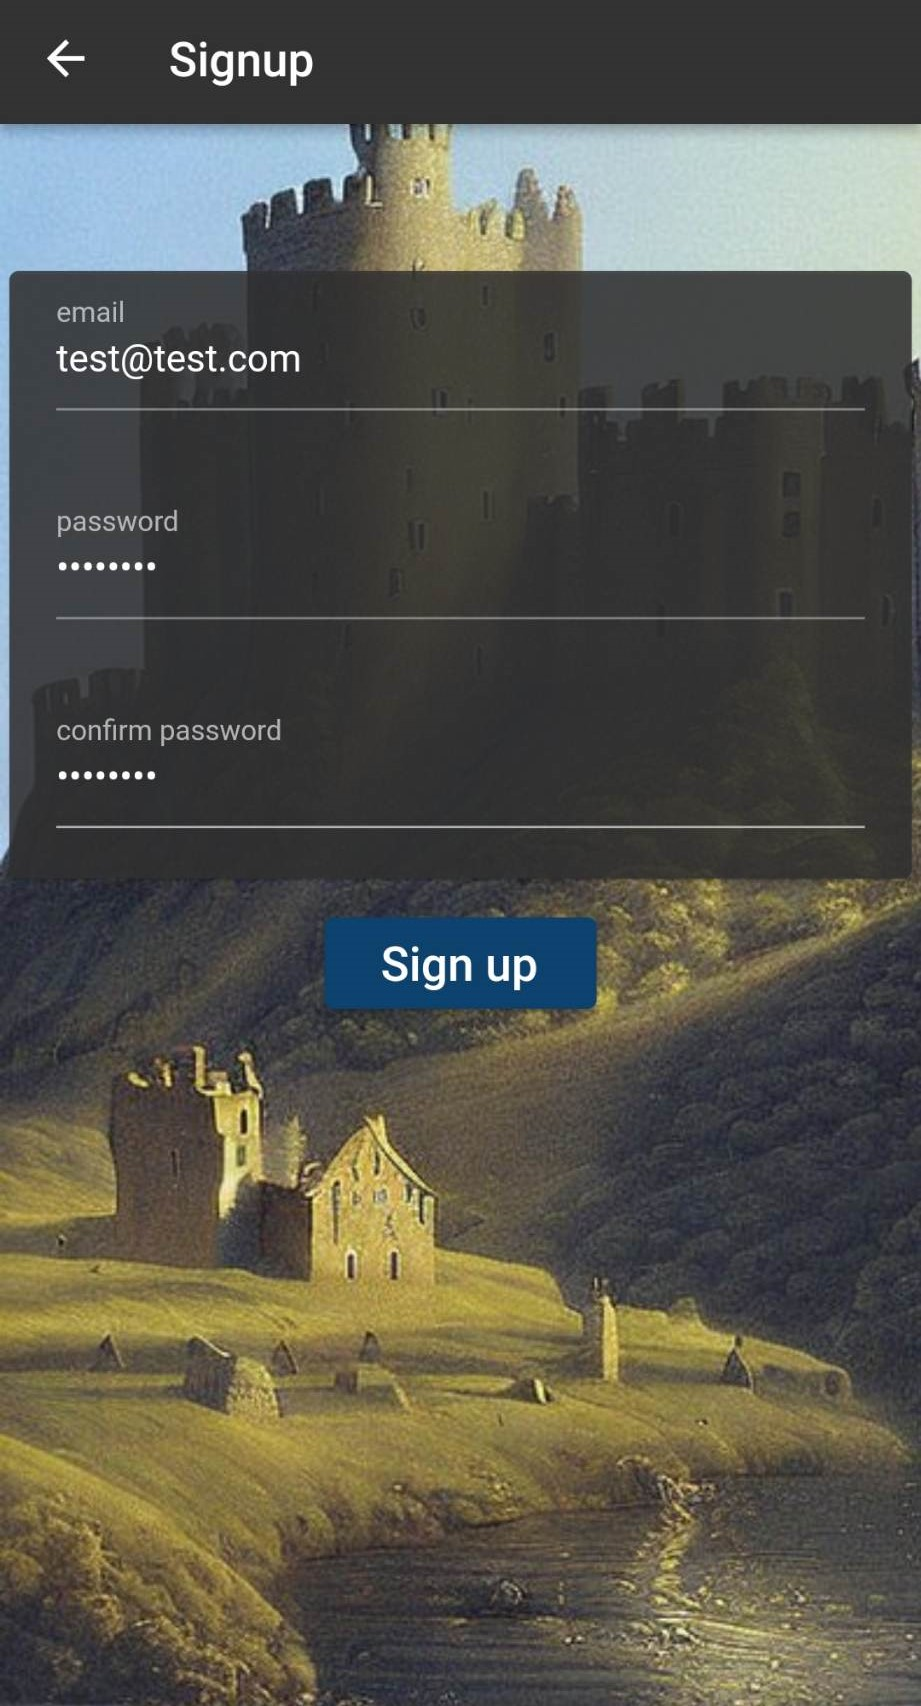
\includegraphics[width=0.4\textwidth]{./img/signup2.jpg}} 
    \centering
\end{figure}
Po wpisaniu email'a oraz hasła i jego powtórzenia użytkownik może kliknąć przycisk rejestracji. Po tym zostanie przekierowany do ekranu Lobby. Może też potem korzystać z utworzonego konta przy zwykłym logowaniu.

Pola tekstowe email i hasło podlegają walidacji. Tworzone hasło powinno mieć co najmniej 8 znaków, w tym literę i cyfrę.

Pola tekstowe email i hasło podlegają walidacji.

\newpage
\subsection{Lobby}
Jeśli użytkownik chce utworzyć nowe konto przechodzi do ekranu rejestracji:
\begin{figure}[!htb]
    \centering
    \subfigure{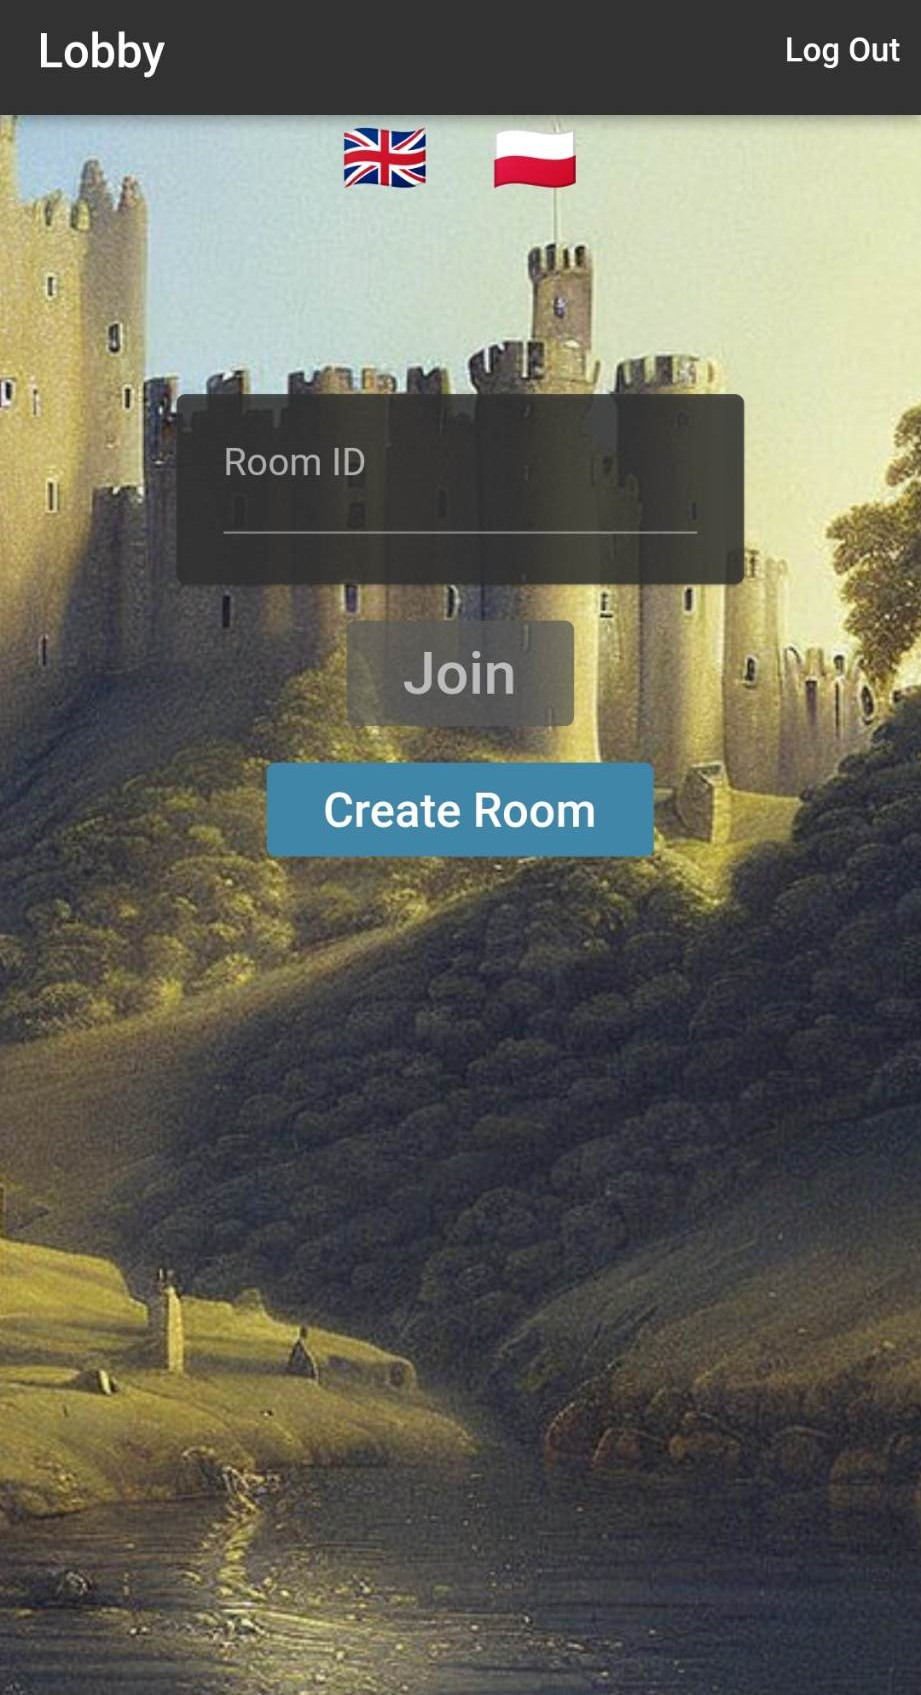
\includegraphics[width=0.4\textwidth]{./img/lobby.jpg}} 
    \subfigure{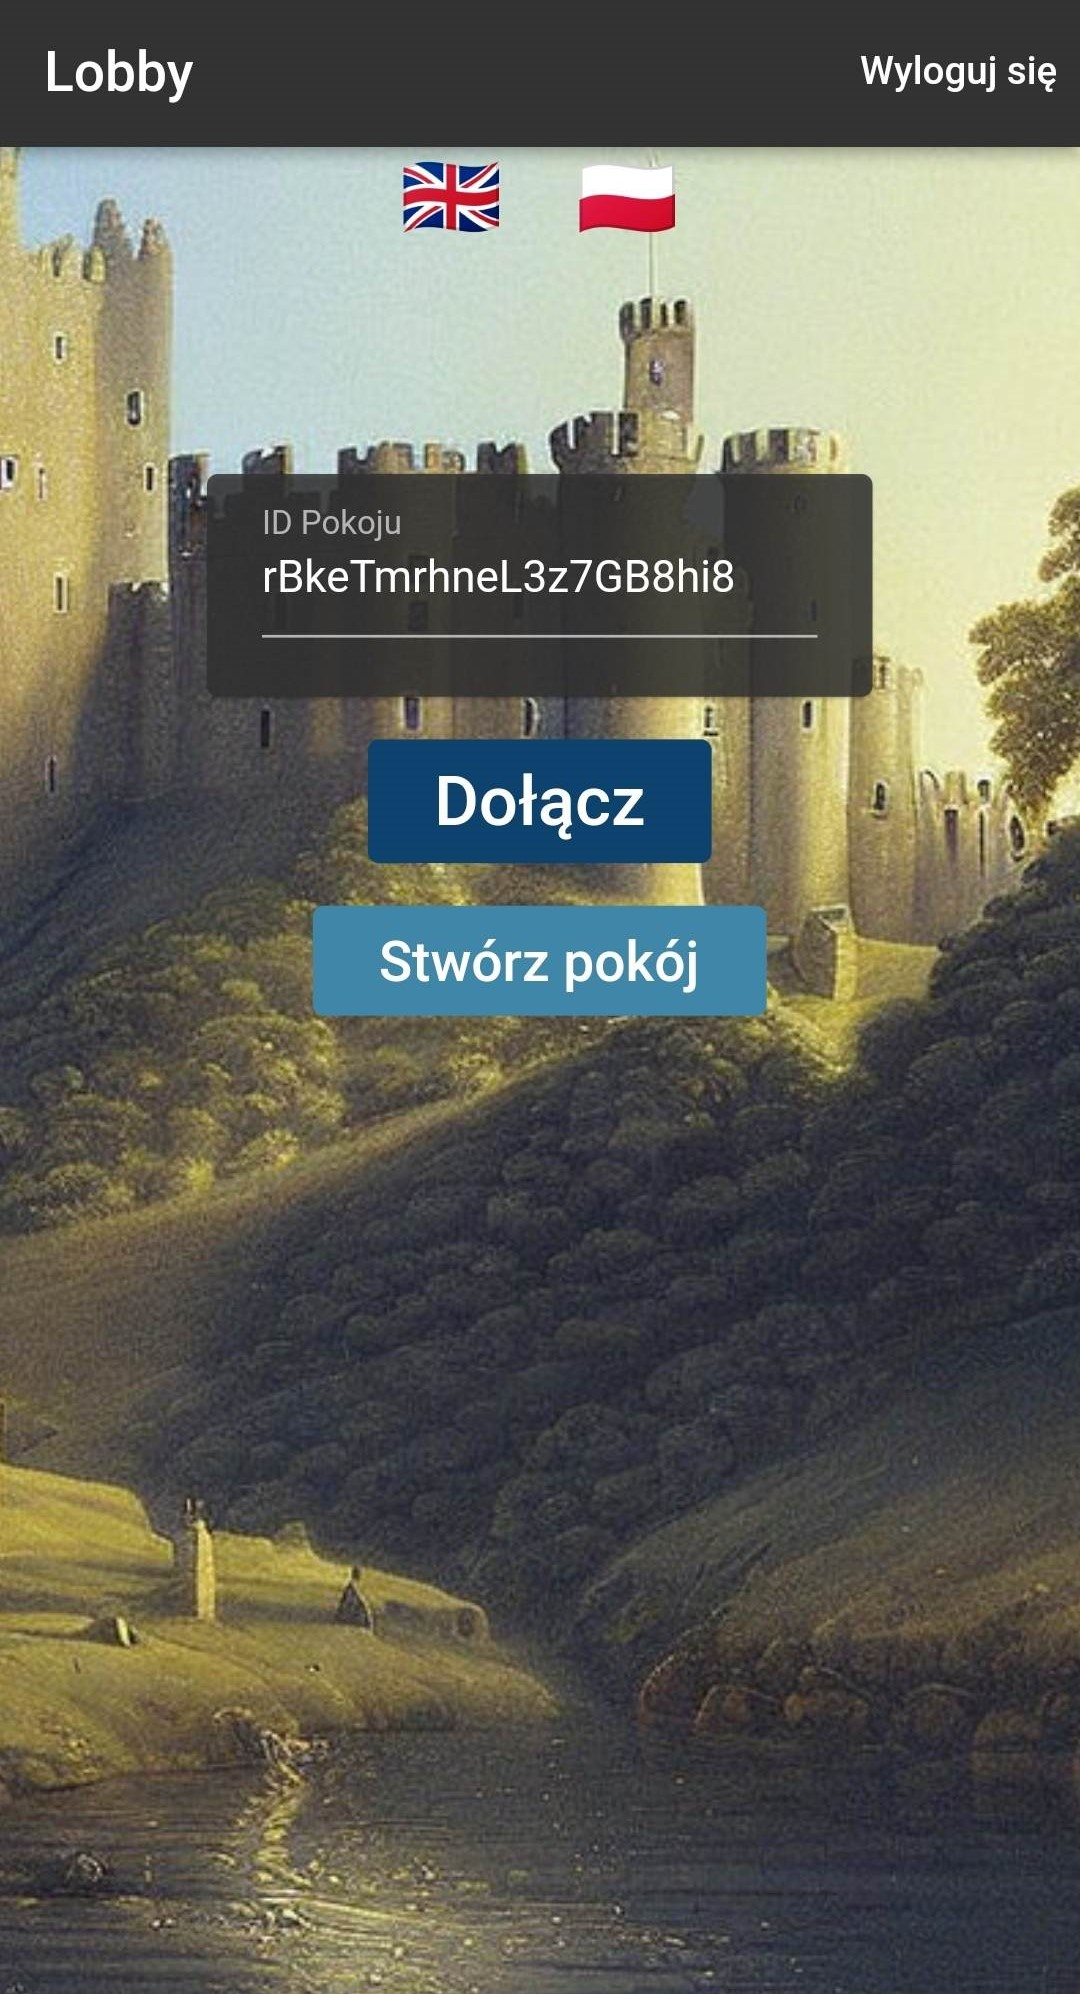
\includegraphics[width=0.4\textwidth]{./img/lobby2.jpg}} 
    \centering
\end{figure}
Użytkownik może:
\begin{itemize}
    \item zmieniać język aplikacji między polskim i angielskim za pomocą przycisków na górze ekranu z flagami. 
    \item wpisać ID pokoju i do dołączyć do niego
    \item stworzyć nowy pokój
    \item wylogować się
\end{itemize}

\newpage
\subsection{Pokój}
Każdorazowo po przejściu do ekranu pokoju użytkownik musi ustalić swój nick, pod którym będzie widoczny na liście graczy.
Po zatwierdzaniu popup znika.
\begin{figure}[!htb]
    \centering
    \subfigure{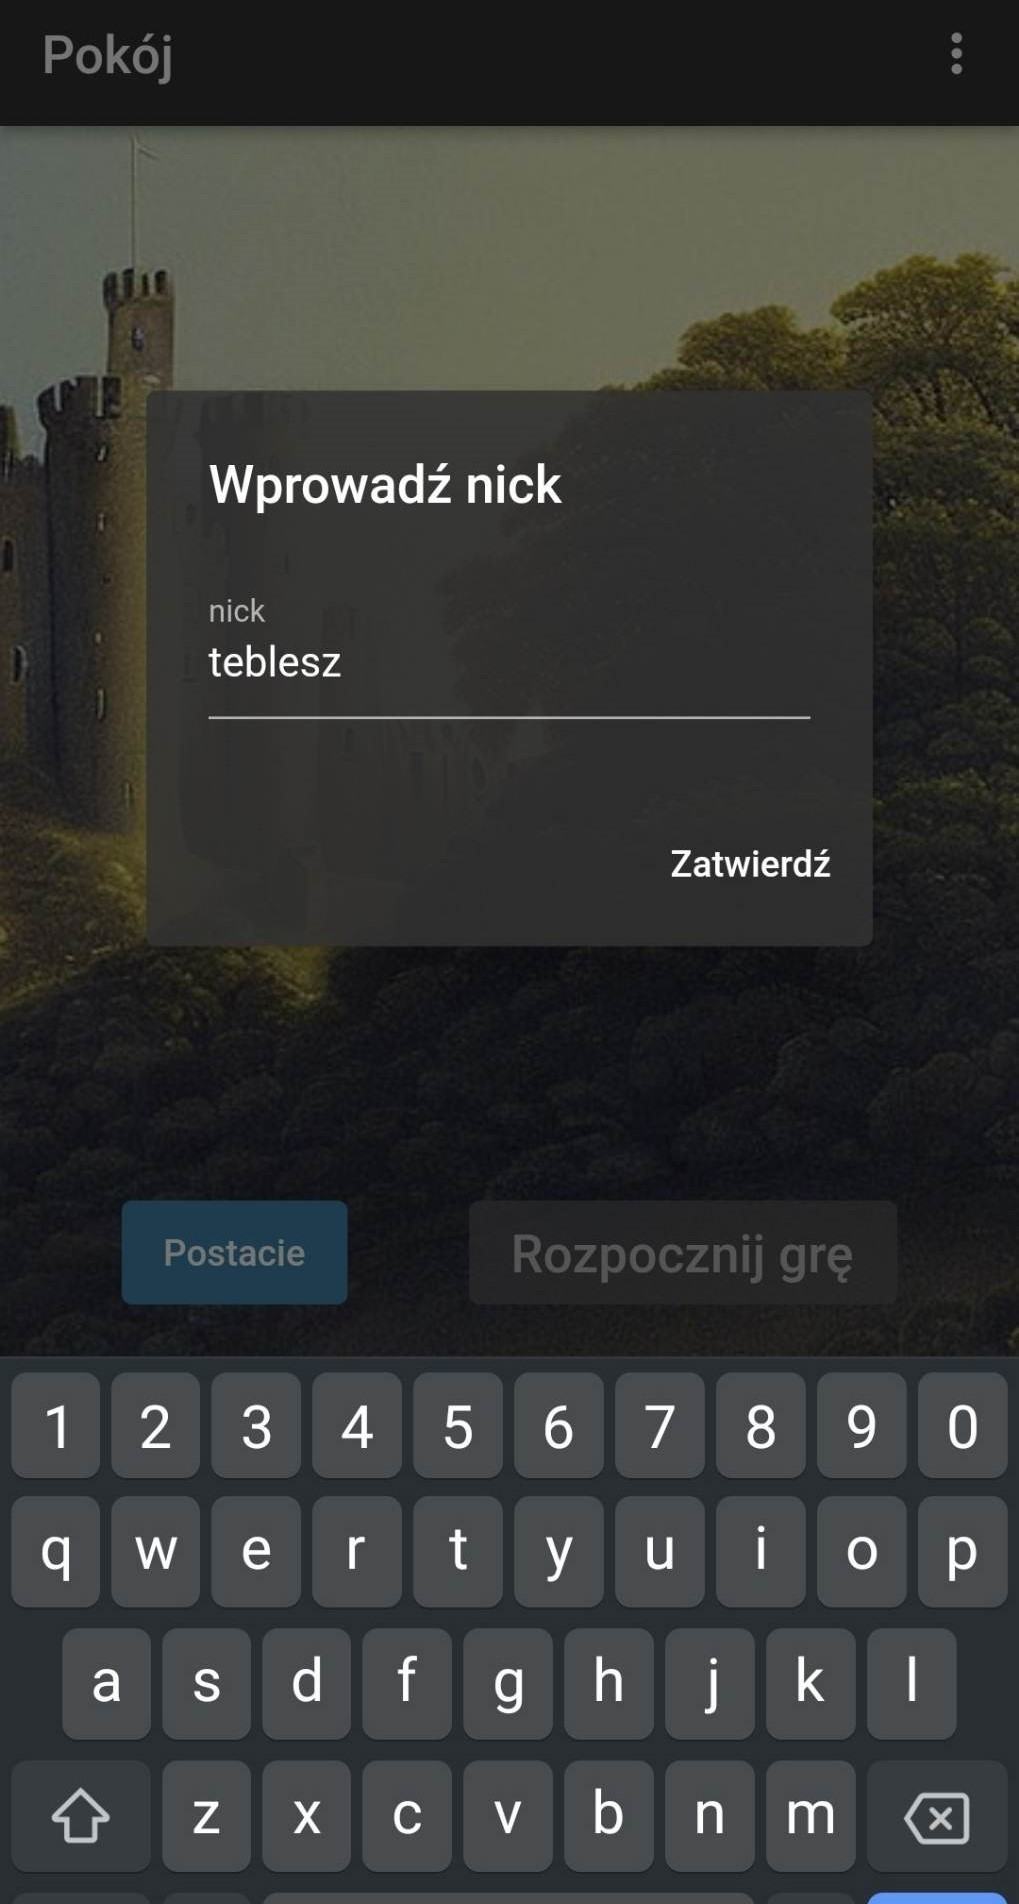
\includegraphics[width=0.3\textwidth]{./img/room_nick.jpg}} 
    \subfigure{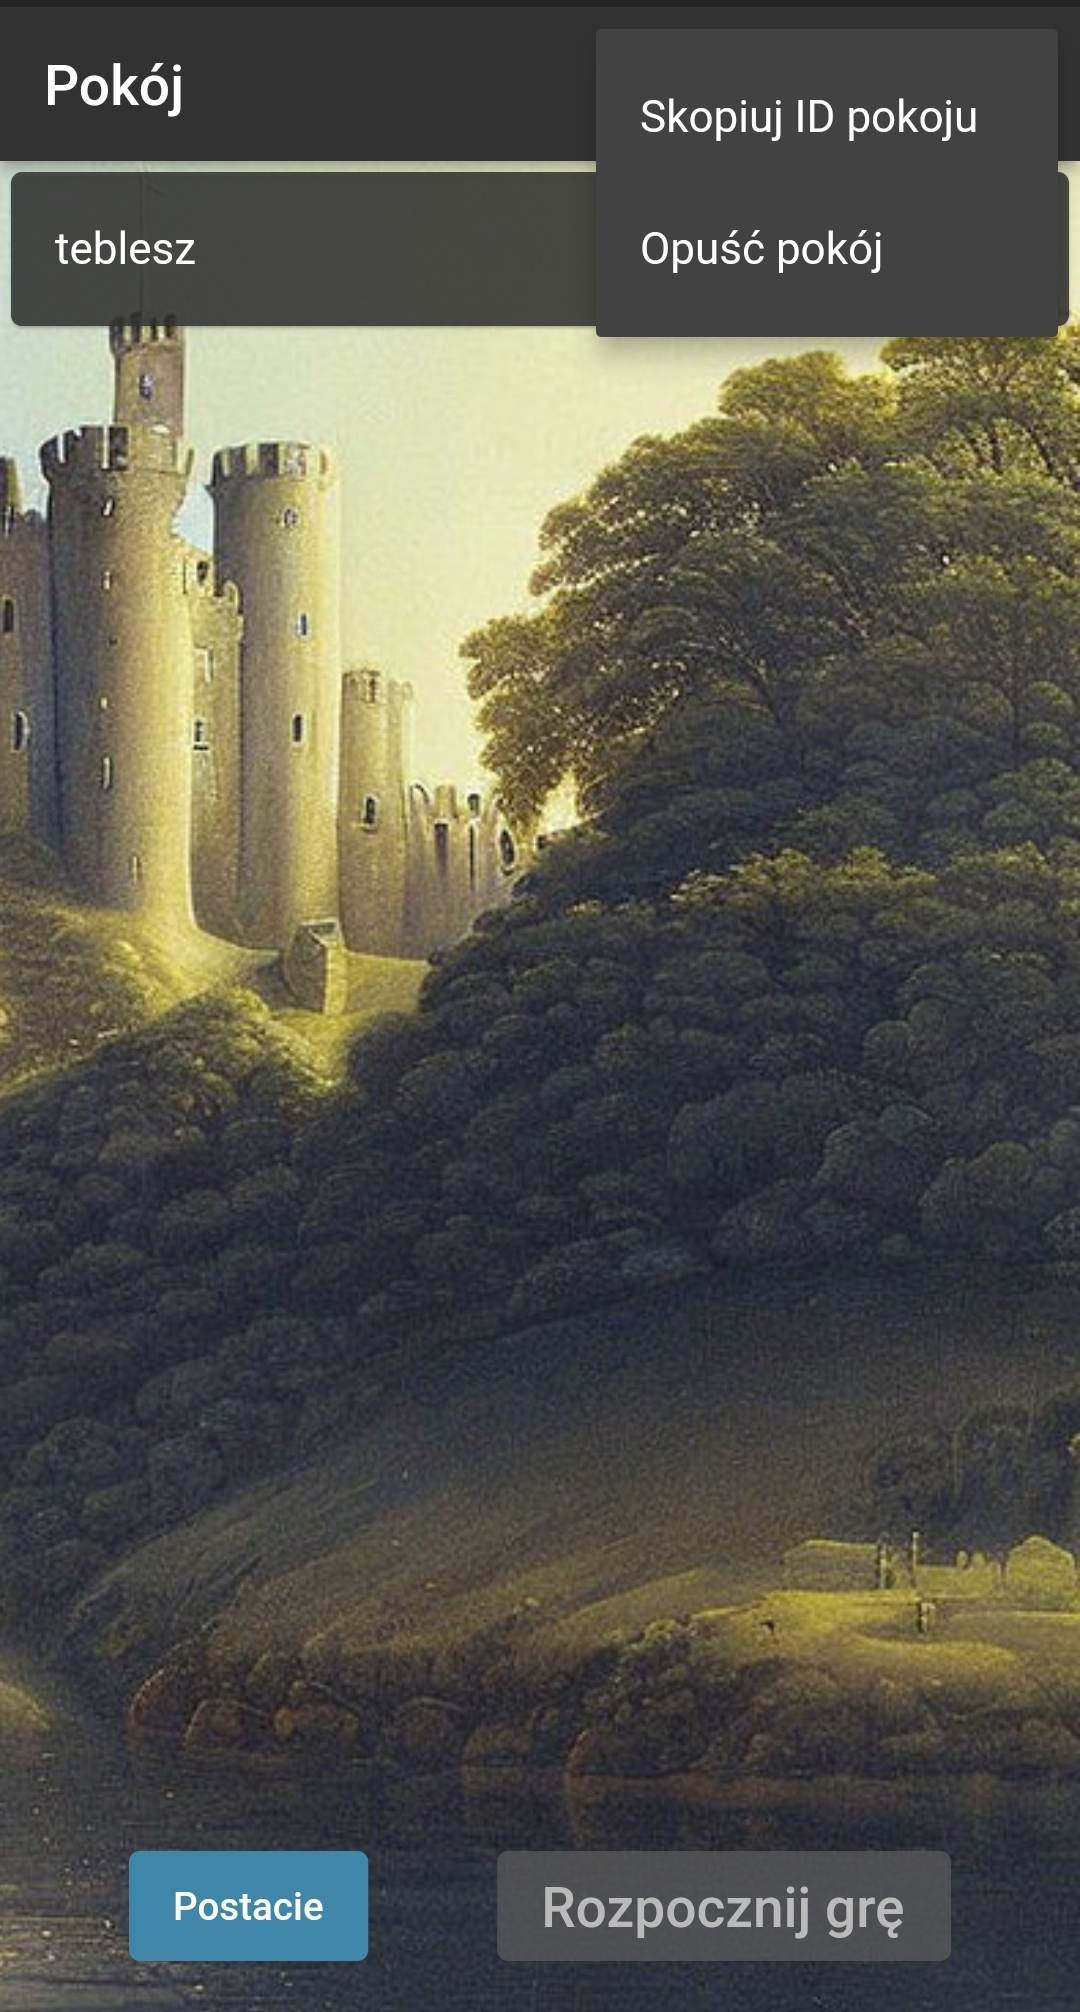
\includegraphics[width=0.3\textwidth]{./img/room_copy.jpg}} 
    \subfigure{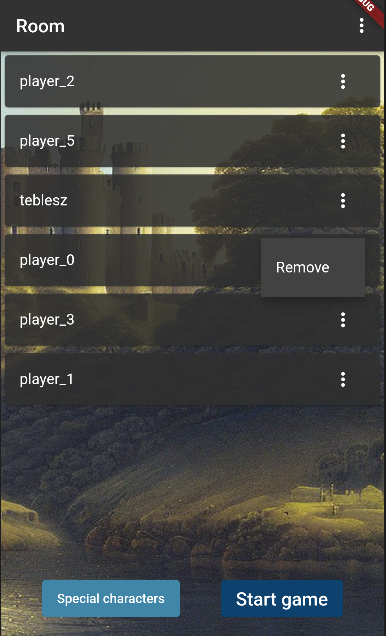
\includegraphics[width=0.3\textwidth]{./img/room5.png}} 
    \centering
\end{figure}

Na ekranie Pokoju Użytkownik może:
\begin{itemize}
    \item w menu pod symbolem trzech kropek skopiować ID pokoju bądź go opuścić
    \item oczekiwać na rozpoczęcie gry przez właściciela pokoju.
\end{itemize}
Użytkownik który utworzył pokój dodatkowo może:
\begin{itemize}
    \item wyrzucać graczy z pokoju klikając na symbol trzech kropek na karcie danego gracza 
    \item modyfikować listę postaci w rozgrywce pod przyciskiem "Postacie".
    \item rozpocząć grę po zgromadzeniu odpowiedniej ilości graczy, tj. co najmniej 5 i co najwyżej 10
\end{itemize}

\begin{itemize}
    \item zmieniać język aplikacji między polskim i angielskim za pomocą przycisków na górze ekranu z flagami. 
    \item wpisać ID pokoju i do dołączyć do niego
    \item stworzyć nowy pokój
    \item wylogować się
\end{itemize}



\newpage
\subsection{Postacie}
Na ekranie postaci właściciel pokoju może definiować jakie postacie dodatkowe wezmą udział w grze.
\begin{figure}[!htb]
    \centering
    \subfigure{
\includegraphics[width=0.4\textwidth]{./img/char1.jpg}} 
    \subfigure{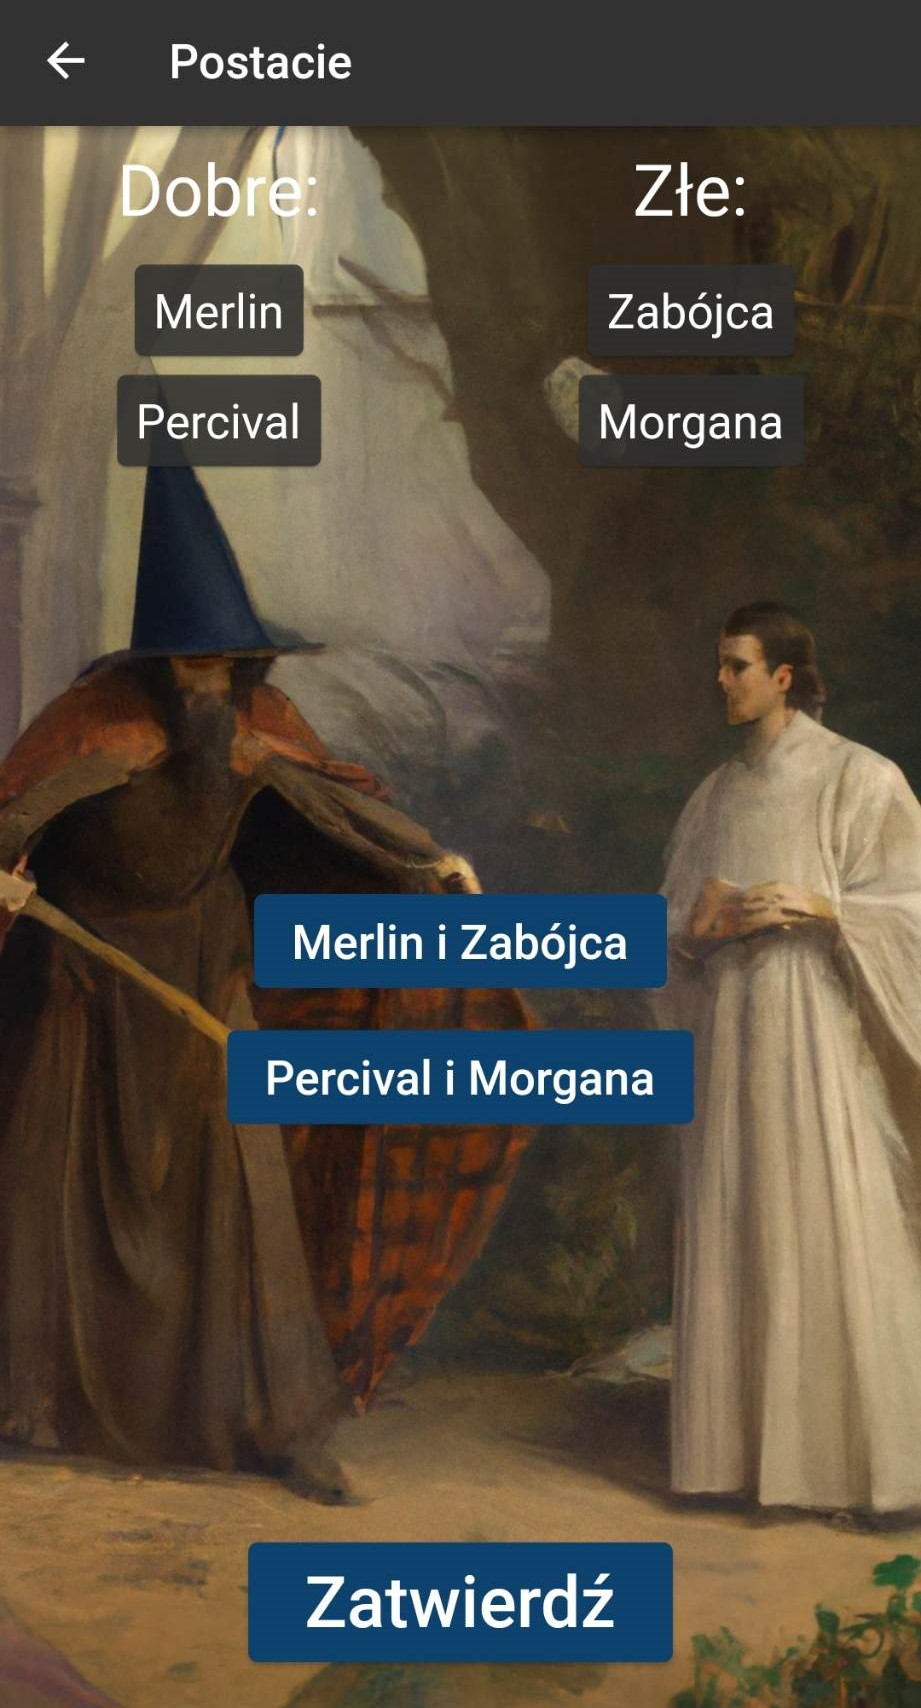
\includegraphics[width=0.4\textwidth]{./img/char2.jpg}} 
    \centering
\end{figure}

Za pomocą przycisków dodaje jedne lub dwa zestawy postaci. Uniemożliwione jest dodanie zestawu Percivala i Morgany jeśli w grze nie ma Merlina i Zabójcy (zgodnie z zasadami gry). Po zdecydowaniu się na którąś wersję rozgrywki właściciel pokoju może zatwierdzić wybór, po czym wraca do ekranu pokoju.


\newpage
\subsection{Gra}
Po rozpoczęciu rozgrywki każdy użytkownik zostanie przekierowany na ekran gry.
\begin{figure}[!htb]
    \centering
    \subfigure{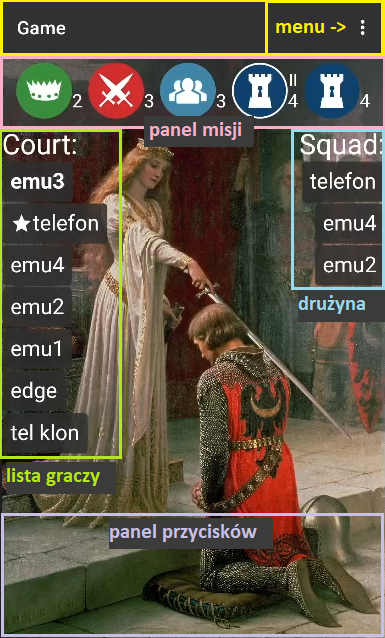
\includegraphics[width=0.5\textwidth]{./img/squad_choice00.png}} 
    \centering
\end{figure}

Ekran gry dzieli się na:
\begin{itemize}
    \item Górny pasek aplikacji - pod menu oznaczonym symbolem trzech kropek użytkownik może wybrać przypomnienie swojej roli lub opuszczenie gry.
    \item Panel misji - wyświetlany jest tu stan każdej z 5-ciu misji gry. Można go odczytać następująco: 
    \begin{itemize}
        \item ciemnoniebieski - przyszła misja
        \item jasnoniebieski - aktualnie rozstrzygana misja
        \item zielony - misja zakończona sukcesem
        \item czerwony - misja zakończona porażką
    \end{itemize}
    Oprócz kolorów paneli widoczne są również reprezentatywne dla stanu misji symbole, oraz liczba reprezentująca liczbę graczy wymaganą dla danej misji. Jeśli jest w białym kole z symbolem II obok niej oznacza to, że wymaga dwóch głosów za porażką (aby zwykła misja zakończyła się porażką wystarczy jeden taki głos).
    \item Lista graczy - lista wszystkich graczy. Lider jest oznaczony gwiazdką, a gracz użytkownika oznaczony pogrubionym fontem nicka. Podczas wyboru drużyny lider wybiera jej członków spośród tej listy poprzez kliknięcie.
    \item Drużyna - lista członków drużyny wybieranej przez lidera. Podczas wyboru drużyny lider może kliknąć na kartę członka drużyny aby go z niej usunąć.
    \item Panel przycisków - w tym miejscu wyświetlane są przyciski:
    \begin{itemize}
        \item Zatwierdzenia drużyny - dostępny dla lidera po wybraniu odpowiedniej dla misji liczby członków drużyny. Rozpoczyna jawne głosowanie.
        \item Przyciski głosowania jawnego - podczas głosowanie wyświetlane są każdemu graczowi, może on wtedy głosować za lub przeciw wybranej przez lidera drużynie.
        \item Przycisk wyruszenia na misję - po zaakaceptowaniu drużyny wyświetlany jest jej członkom i przekierowuje ich do ekrany głosowania tajnego.
    \end{itemize}
\end{itemize}

W poniższych sekcjach ukazane są ekrany widoczne podczas przebiegu gry.

\subsubsection{Start gry}
\begin{figure}[!htb]
    \centering
    \subfigure{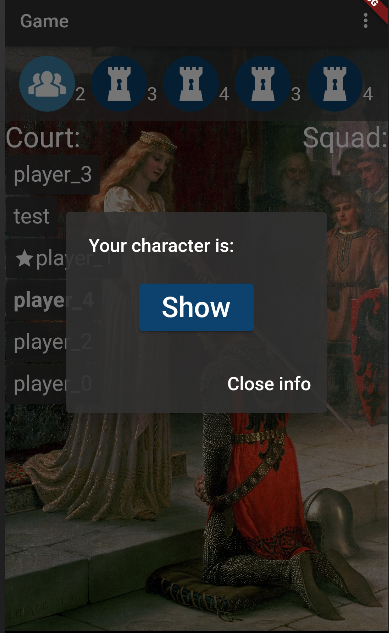
\includegraphics[width=0.305\textwidth]{./img/start0.png}} 
    \subfigure{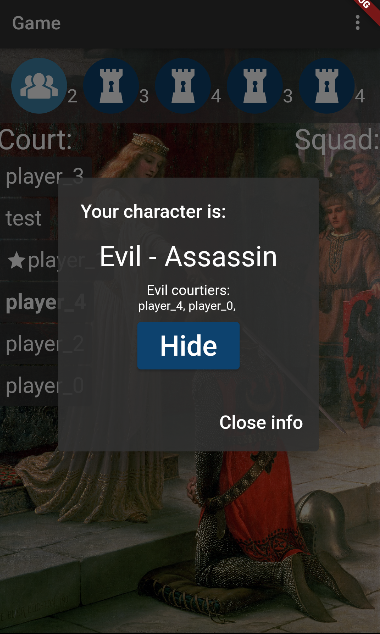
\includegraphics[width=0.3\textwidth]{./img/start1.png}} 
    \subfigure{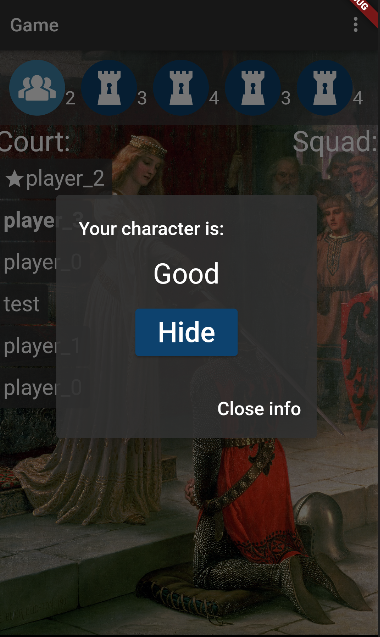
\includegraphics[width=0.3\textwidth]{./img/start2.png}} 
    \centering
\end{figure}
Po rozpoczęciu gry gracz widzi jaka rola została mu przydzielona, wraz z możliwie przydzieloną postacią (po myślniku). Źli gracze widzą dodatkowo informację o tym kto jest Złymi podczas tej gry. Informacje są ukryte za przyciskiem, aby zachować ich niejawność.

Okno dialogowe można zamknąć przyciskiem na dole.
W razie zapomnienia roli przez gracza to samo okno pokaże się po kliknięciu jednej z opcji w menu na górze ekranu (pod symbolem trzech kropek).

\subsubsection{Wybór drużyny}
Na poniższych trzech obrazach ukazano widok lidera podczas wyboru drużyny. Na początku drużyna jest pusta, potem dodany zostaje jedne z graczy. Następnie dodany został drugi gracz. Ta liczba graczy pokrywa się ze wskazaną obok kafelka misji liczbą więc lider może kliknąć przycisk zatwierdzenia drużyny na dole ekranu.
\begin{figure}[!htb]
    \centering
    \subfigure{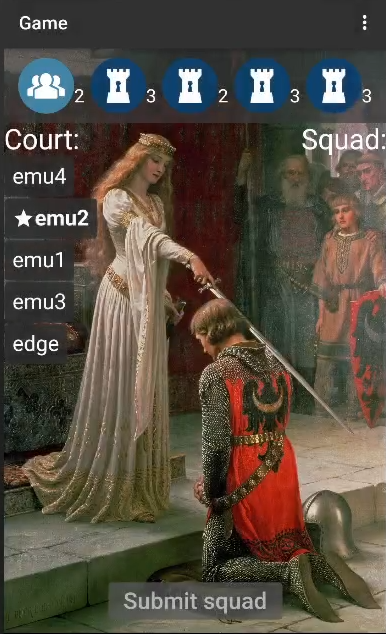
\includegraphics[width=0.3\textwidth]{./img/choice1.png}} 
    \subfigure{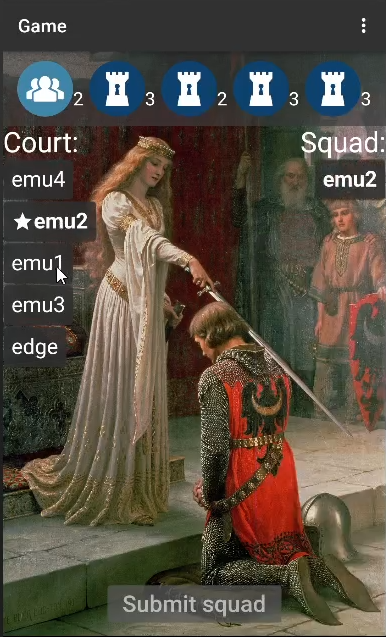
\includegraphics[width=0.3\textwidth]{./img/choice2.png}} 
    \subfigure{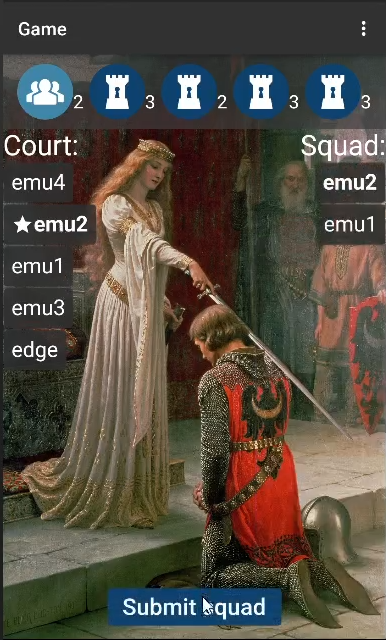
\includegraphics[width=0.3\textwidth]{./img/choice3.png}} 
    \centering
\end{figure}

\subsubsection{Głosowanie jawne na drużynę}
Drużyna podlega teraz głosowaniu wszystkich graczy. Jeśli większość graczy zagłosuje "za" na panelu u dołu ekranu (przyciski czerwony i zielony dezaktywują się po kliknięciu) to drużyna zostaje zaakceptowana i następuje przejście do głosowania - członkowie drużyny mogą wyruszyć na misję z tajnym głosowaniem (niebieski przycisk na dole ekranu - dezaktywowany po oddaniu głosu tajnego).
W przeciwnym przypadku drużyna nie zostaje zaakceptowana, następuje przejście do następnego lidera, który wybiera nową drużynę.
\begin{figure}[!htb]
    \centering
    \subfigure{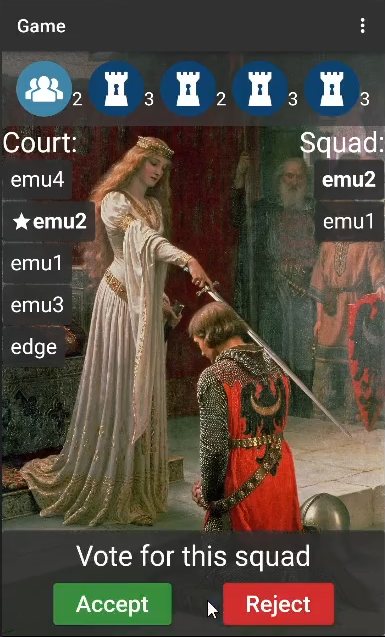
\includegraphics[width=0.35\textwidth]{./img/vote1.png}} 
    \subfigure{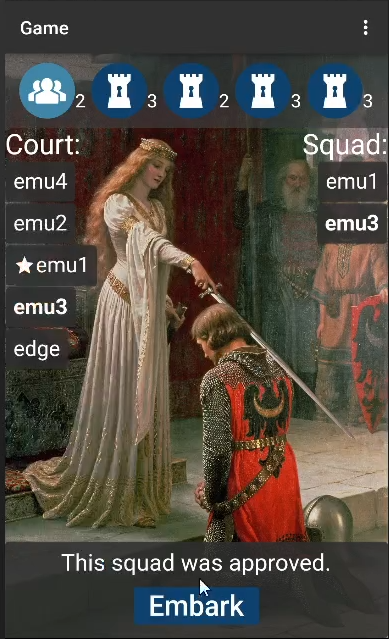
\includegraphics[width=0.35\textwidth]{./img/embark1.png}} 
    \centering
\end{figure}


\newpage
\subsubsection{Głosowanie tajne na misji}
Po kliknięciu przycisku wyruszenia członkowie drużyny przechodzą do ekranu głosowania tajnego. 
\begin{figure}[!htb]
    \centering
    \subfigure{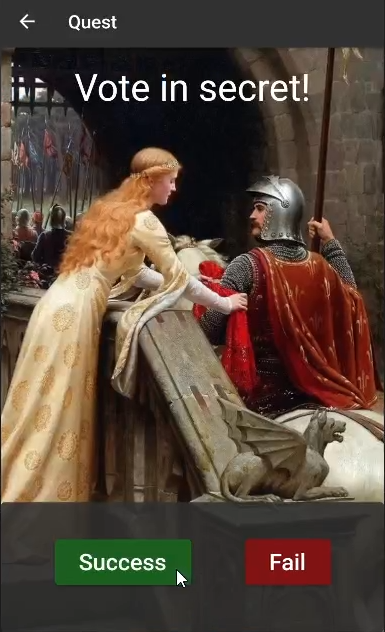
\includegraphics[width=0.42\textwidth]{./img/vote2.png}} 
    \centering
\end{figure}

Dobrzy gracze mogą głosować tylko za sukcesem misji (klikanie przycisku porażki nie wywołuje żadnej akcji), natomiast źli gracze mogą głosować za sukcesem lub za porażką. Wg. zasad gry wystarczy jeden głos za porażką aby misja się nie powiodła.

Przyciski są ustawione losowo, tj. przy każdorazowym otworzeniu tego ekranu to który przycisk jest z lewej, a który z prawej jest losowane. ekran można zamknąć strzałką powrotu w jego lewym górnym kącie a następnie do niego wrócić przyciskiem wyruszenia, a ustawienie zostanie wylosowane raz jeszcze. Umożliwia to głosowanie w sekrecie nawet jeśli ktoś podgląda gdzie celuje nas palec, lub zobaczył pierwotny układ przycisków na naszym ekranie.

\subsubsection{Wynik misji}
Po tym jak wszyscy członkowie drużyny zagłosują, wszystkim graczom pokazywane jest okno z wynikiem misji i odpowiednio zmienia się wygląd panelu misji.
\begin{figure}[!htb]
    \centering
    \subfigure{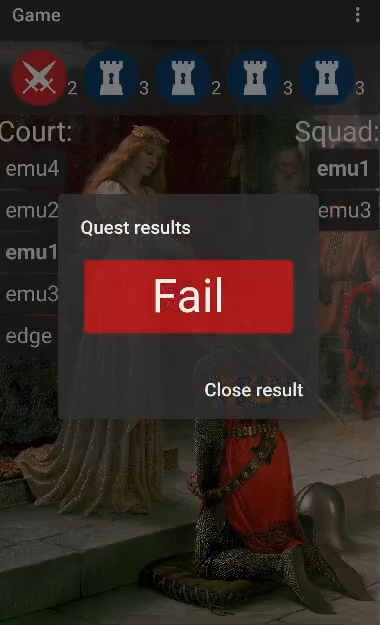
\includegraphics[width=0.4\textwidth]{./img/result1.png}} 
    \subfigure{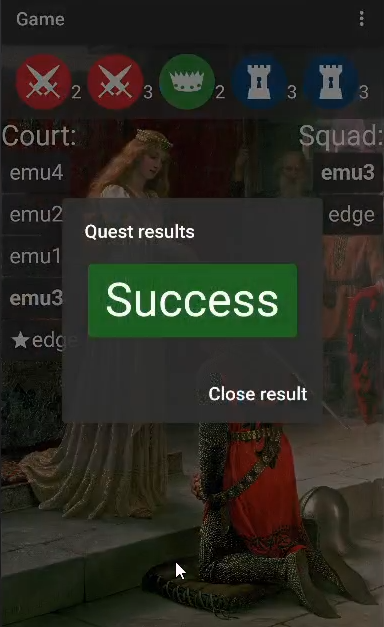
\includegraphics[width=0.4\textwidth]{./img/result2.png}} 
    \centering
\end{figure}
Jeśli w trakcie gry były 3 misje zakończone sukcesem lub 3 misje zakończone porażką to po zamknięciu tego okna pojawi się okno z wynikiem gry.
W przeciwnym przypadku rozgrywka wraca do etapu wybory drużyny z nowym liderem i nową drużyną.



\newpage
\subsubsection{Wynik gry}
Okno zakończenia gry informuje graczy o wygranej Dobrych lub wygranej Złych. 
Wszyscy dowiadują się także, którzy gracze byli źli.

Jeżeli w grze był Merlin i Zabójca to po wygranej dobrych, gracz będący zabójcą może wybrać z listy graczy, tego kogo uważa za Merlina. Jeśli trafił dobrze to wynik gry się zmienia i to Źli wygrywają.
\begin{figure}[!htb]
    \centering
    \subfigure{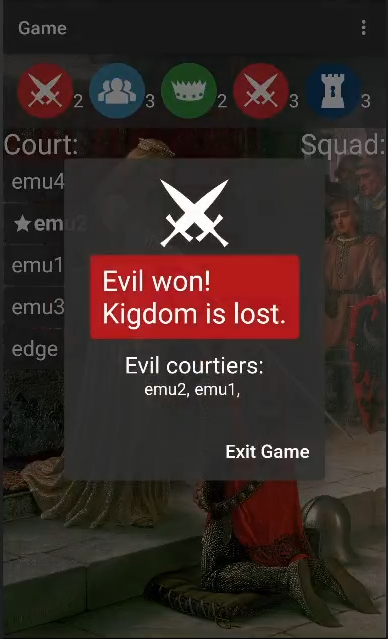
\includegraphics[width=0.3\textwidth]{./img/result12.png}} 
    \subfigure{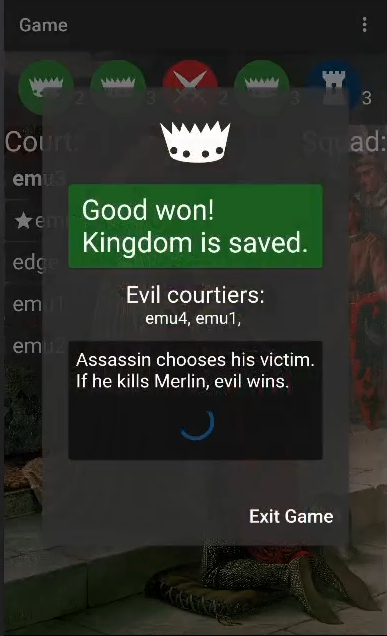
\includegraphics[width=0.3\textwidth]{./img/result10.png}} 
    \subfigure{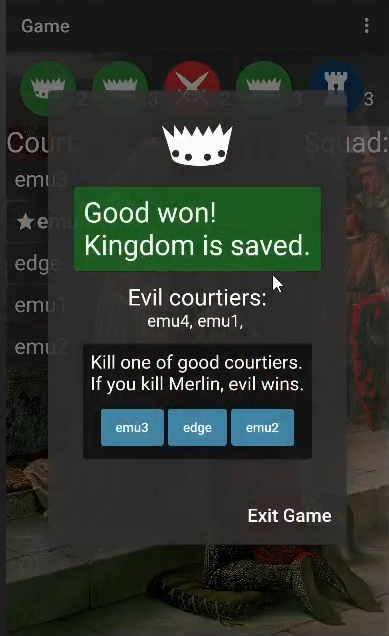
\includegraphics[width=0.3\textwidth]{./img/result11.png}} 
    \centering
\end{figure}
\begin{itemize}
    \item Na pierwszym obrazku przedstawiono wariant z wygraną złych.
    \item Na drugim widać wariant z wygraną dobrych i oczekiwanie na to kogo wybierze zabójca.
    \item Trzeci ekran widzi tylko zabójca - może wybrać którego gracza zabija.
    \item Na Czwartym ekranie widać ostateczny wynik gry
\end{itemize}
Jedynym co może kliknąć gracz po zakończeniu gry to przycisk wyjścia z pokoju, który wraca go do ekranu Lobby, gdzie może dołączyć do nowego pokoju.




\newpage
\section{Schemat bazy danych}
Poniżej na rysunku \ref{modele} przedstawiony został schemat bazy danych \textbf{Firestore}. Użyto diagramu klas aby lepiej zobrazować kolekcje dokumentów utworzonych w tej nierelacyjnej bazie danych. Każda klasa stanowi wzór dokumentu odpowiadającej kolekcji. Pola o typie \texttt{typ?} są opcjonalne.
\begin{figure}[!htb]
    \centerline{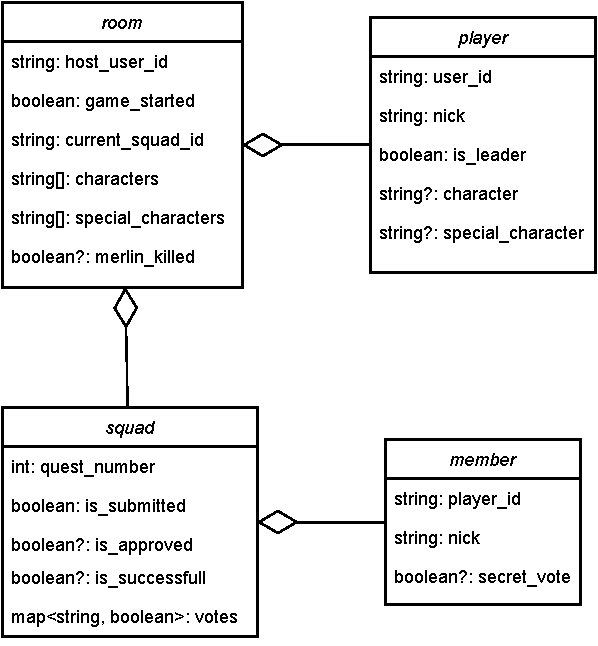
\includegraphics[width=0.8\textwidth]{./img/modele.pdf}}
    \caption{Schemat bazy danych Firestore}
    \centering
    \label{modele}
\end{figure}


\newpage
\section{CI/CD}
Poniżej przedstawiono zawartość pliku \texttt{android\_release.yaml} odpowiedzialnego za stworzenie wersji release aplikacji dla Androida. 

\begin{minted}[
    frame=single,
    framesep=2mm,
]{yaml}
name: Android Release

on:
  push:
    branches: [ "main" ]
  pull_request:
    branches: [ "main" ]

  workflow_dispatch:

jobs:
  build:
    runs-on: ubuntu-latest

    steps:
      - uses: actions/checkout@v3
      - uses: actions/setup-java@v3
        with:
          distribution: 'zulu'
          java-version: "12.x"
          cache: 'gradle'
      - uses: subosito/flutter-action@v2
        with:
          flutter-version: "3.7.0"
          channel: 'stable'
          cache: true
      - name: Get dependencies
        run: flutter pub get

      - name: Generate Localization files
        run: flutter gen-l10n

      - name: Build app
        run: flutter build apk
      - uses: actions/upload-artifact@v1
        with:
          name: release-apk
          path: build/app/outputs/apk/release/app-release.apk
\end{minted}

\newpage
Poniżej przedstawiono zawartość pliku \texttt{web-deployment.yaml} odpowiedzialnego za stworzenie wersji release aplikacji dla storny web i jej opublikowanie. 


\begin{minted}[
    frame=single,
    framesep=2mm,
]{yaml}
name: Web Deployment

on:
  push:
    branches: [ "main" ]
  pull_request:
    branches: [ "main" ]
    
jobs:
  build:
    name: Build Web
    env:
      my_secret: ${{secrets.commit_secret}}
    runs-on: ubuntu-latest
    steps:
      - uses: actions/checkout@v3 
      - uses: subosito/flutter-action@v2
        with:
          flutter-version: "3.7.0"
          channel: 'stable'
          cache: true
      - run: flutter config --enable-web
      - run: flutter pub get
      - run: flutter gen-l10n
      - run: flutter build web --release
      - run: |
          cd build/web
          git init
          git config --global user.email mteblesz@gmail.com
          git config --global user.name teblesz
          git status
          git remote add origin https://${{secrets.commit_secret}}\ 
          @github.com/teblesz/fluttartur.git
          git checkout -b gh-pages
          git add --all
          git commit -m "update"
          git push origin gh-pages -f
\end{minted}


\newpage
\section{Użyte grafiki}
Dla rozwiania możliwych wątpliwości dot. praw autorskich:
\begin{itemize}
    \item 
\includegraphics[width=0.1\textwidth]{./img/icon.png} ikona aplikacji została wygenerowana przez model DALL-E 
    
    \url{https://labs.openai.com/}

    \item grafika w tle ekranów Logowania, Rejestracji, Lobby i Pokoju oraz grafika w tle ekranu Postaci zostały wygenerowane przez model Stable Diffusion 
    
    \url{https://stablediffusionweb.com/#demo}
    \item grafiki w tle ekranów Gry i Misji to obrazy malarza Edmunda Blair'a Leightona (zm. 1922). Grafika ekranu misji została rozszerzona poza oryginalne krawędzie używając narzędzia DALL-E.
\end{itemize}



\section{Linki projektu}
\begin{itemize}
    \item 
    Aplikacja jest dostępna do pobrania pod linkiem: \\
    \url{https://github.com/teblesz/fluttartur/suites/12834898379/artifacts/691437348} lub wersja skompilowana lokalnie pod adresem \url{http://bitly.pl/chcUC}
    \item Repozytorium projektu - \url{https://github.com/teblesz/fluttartur}
    \item Strona web z aplikacją na GitHub Pages - \url{https://teblesz.github.io/fluttartur}
\end{itemize}

\end{document}